\chapter{Results and Discussion}\label{chap:results_discussion}

In this thesis, our main focus was on binary classification models. While we did explore regression models, the primary findings we gained stemmed from the analysis and evaluation of classification models. We have omitted the results of the regression evaluation in this chapter as the central contributions lie within the domain of classification.

\section{Binary Classification}
The objective is to maximize the probability of detecting toxic compounds (true positive rate) while minimizing the the number of false alarms, which are non-hazardous compounds misclassified as toxic (false positive rate). We first present which metrics we used to evaluate the performance of the models. Then, we present the performance results for the binary classification models.

\subsection{Evaluation Metrics}
When assessing the performance of a binary prediction model using a validation dataset containing known target values, four key quantities come into play:

\begin{itemize}
  \item True Positives (TP): The number of correctly predicted active cases.
  \item True Negatives (TN): The number of correctly predicted inactive cases.
  \item False Positives (FP): The number of incorrectly predicted active cases.
  \item False Negatives (FN): The number of incorrectly predicted inactive cases.
\end{itemize}

With these four values, a confusion matrix can be created, as shown in Table~\ref{tab:confusion_matrix}.

\begin{table}[h]
  \centering
  \caption{Confusion Matrix}
  \label{tab:confusion_matrix}
  \setlength{\tabcolsep}{10pt} % Adjust cell padding
  \renewcommand{\arraystretch}{1.5} % Adjust cell height
  \begin{tabular}{|c|c|c|}
  \cline{2-3}
  \multicolumn{1}{c|}{} & Actual Negative & Actual Positive \\
  \hline
  Predicted Negative & TN & FN \\
  \hline
  Predicted Positive & FP & TP \\
  \hline
  \end{tabular}
\end{table}

In binary classification, the classification threshold is a crucial parameter dictating how the model assigns data points to one of two classes based on predicted class probabilities. This threshold significantly influences the model's metrics, as illustrated in Figure~\ref{fig:classification_threshold} and exemplified in Figure~\ref{fig:roc1120} and Figure~\ref{fig:cm1120}.
\begin{figure} 
  \centering
  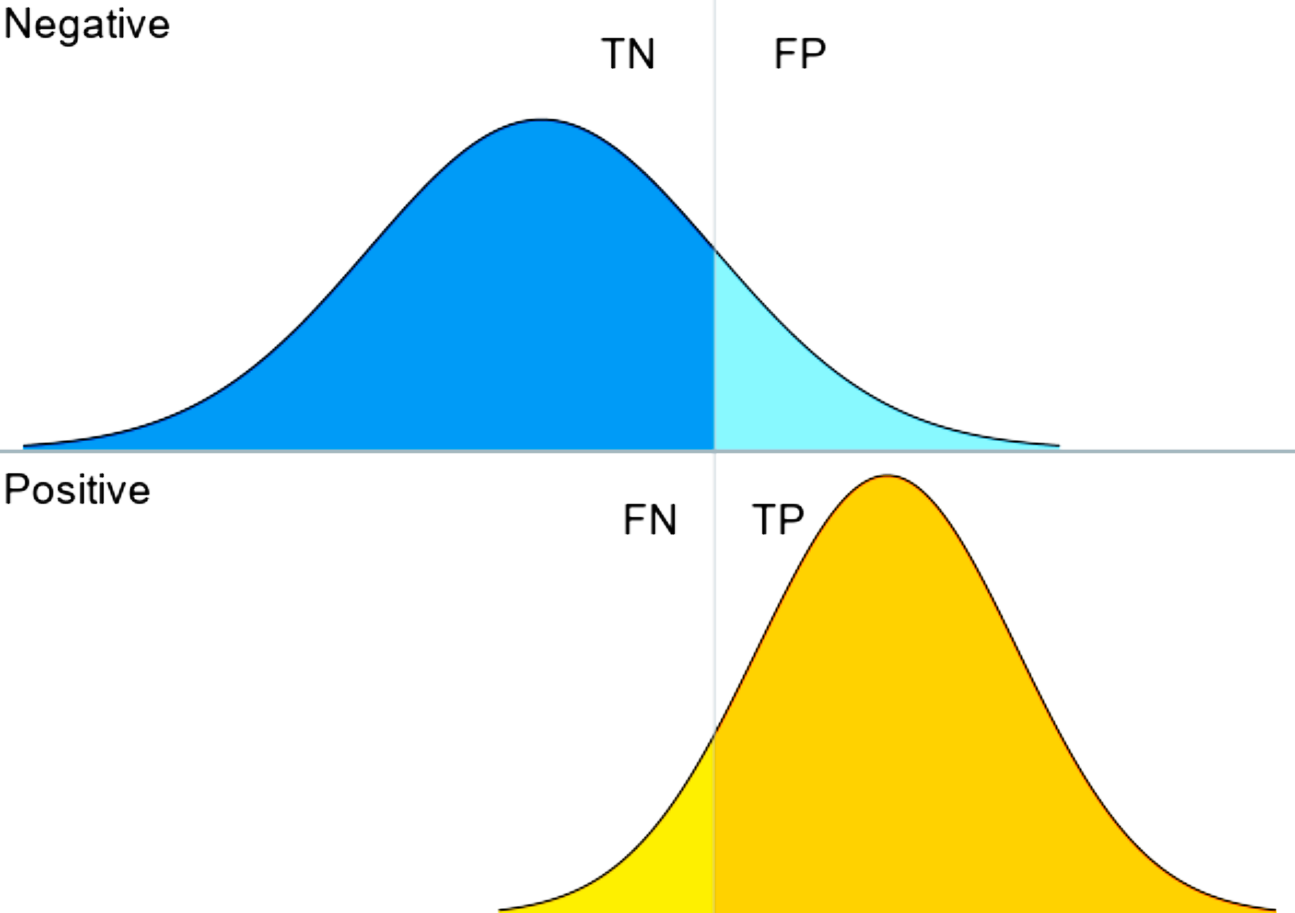
\includegraphics[width=0.5\textwidth]{figures/classification_threshold.png}
  \caption{Relationship between threshold and classification. Figure obtained from~\cite{wicklin2020}}
~\label{fig:classification_threshold}
\end{figure}

Various metrics assess predictive model performance, such as:

\begin{itemize}
  \item \textbf{Accuracy} is the ratio of correctly classified instances (TP) and (TN) to the total number of instances. It provides a general measure of the model's correctness.
  \[ \text{Accuracy}  A = \frac{TP + TN}{TP + TN + FP + FN} \]

  \item \textbf{Precision (P)} is the proportion of correctly predicted active cases (TP) to all instances predicted as active (TP + FP). 
  \[ \text{Precision } P = \frac{TP}{TP + FP} \]

  \item \textbf{Recall (R) or Sensitivity or True Positive Rate (TPR)} is the proportion of correctly predicted active cases (TP) to all actual active cases (TP + FN).
  \[ \text{Recall } R = \frac{TP}{TP + FN} \]

  \item \textbf{F1 Score} is the harmonic mean of precision and recall, which balances the trade-off between false positives and false negatives.
  \[ F1 = \frac{2 \cdot P \cdot R}{P + R} \]

  \item \textbf{True Negative Rate (TNR) or Specificity} is the proportion of correctly predicted inactive cases (TN) to all actual inactive cases (TN + FP).
  \[ TNR = \frac{TN}{TN + FP} \]

  \item \textbf{Receiver Operating Characteristic (ROC) Curve} is a graphical representation of the model's performance across different classification thresholds and plots the true positive rate (TNR) against the false positive rate (FPR), as exemplified for assay endpoint with aeid: 1120 in Figure~\ref{fig:roc1120}. The Area Under the ROC Curve (AUC) is an indicator of the model's performance taking into acount all possible classification thresholds, where a score of 1 represents a perfect model and 0.5 signifies a random no-skill model. 


\end{itemize}

The following two metrics are not directly dependent on the classification threshold, and thus are well-suited for comparing models with imbalanced datasets:

\begin{itemize}
  \item \textbf{Balanced Accuracy (BAC)} accounts for class imbalance by averaging the true positive rate (sensitivity) and true negative rate (specificity).
  \[ \text{Balanced Accuracy (BAC)} = \frac{1}{2} \left(\frac{TP}{TP + FN} + \frac{TN}{TN + FP}\right) \]

  \item \textbf{PR-AUC (Precision-Recall Area Under the Curve)} quantifies the performance of the positive class by assessing the area under the precision-recall curve.
  
\end{itemize}


\begin{figure}[h]
  \centering
  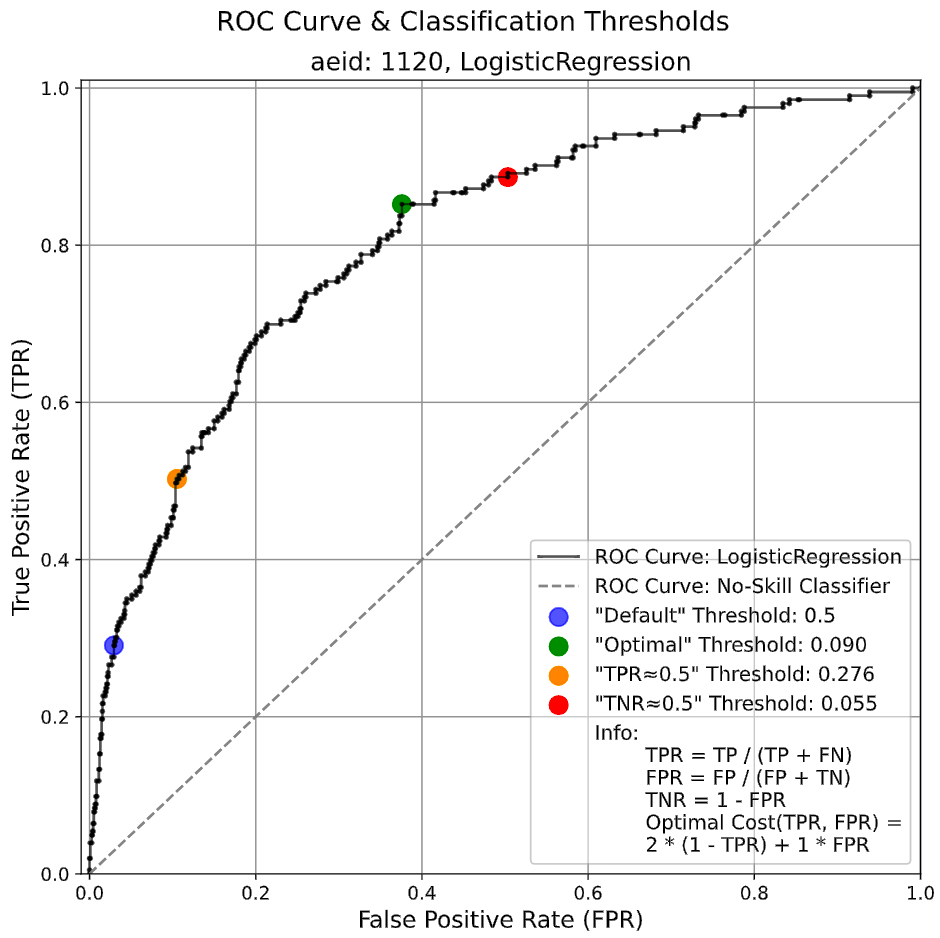
\includegraphics[width=0.7\textwidth]{figures/roc1120.png}
  \caption{The Receiver Operating Characteristic (ROC) curve is presented for the LogisticRegression classifier in the case of assay endpoint with aeid: 1120. We make predictions for each model combination using four distinct classification thresholds, specifically: the default threshold of 0.5, the optimal threshold determined by the cost function weighting TPR twice as FPR (to value recall), TPR approximately equal to 0.5, and TNR approximately equal to 0.5. Figure~\ref{fig:cm1120} shows the confusion matrices for the four thresholds.}
~\label{fig:roc1120}
\end{figure}

\begin{figure}[h]
  \centering
  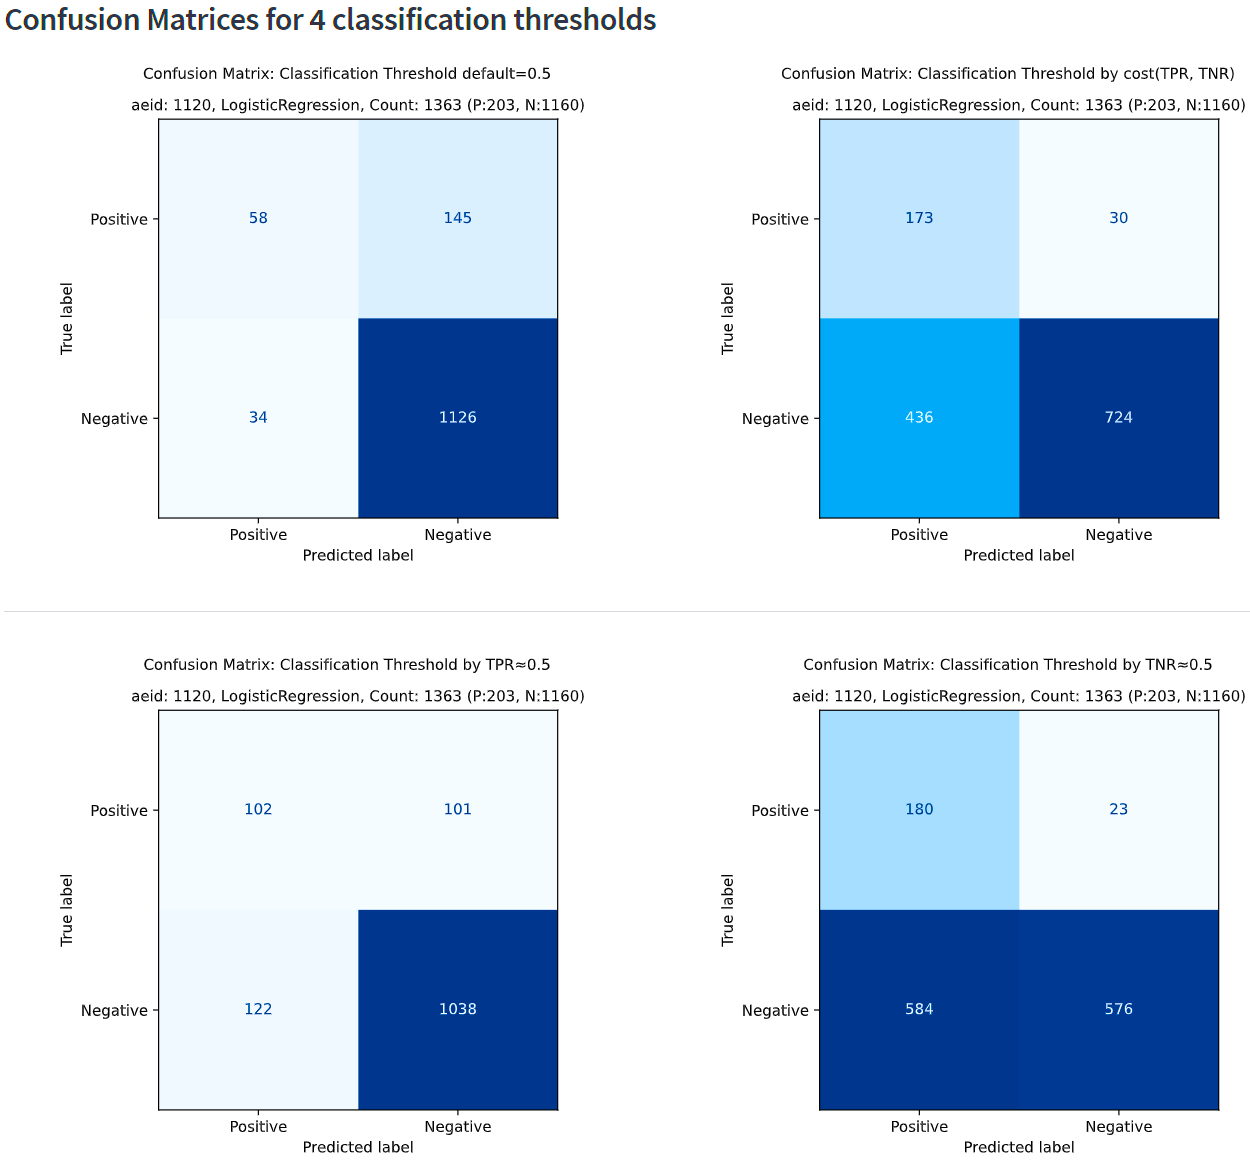
\includegraphics[width=1.0\textwidth]{figures/cm1120.png}
  \caption{For assay endpoint with aeid: 1120, confusion matrices are shown for four different classification thresholds.}
~\label{fig:cm1120}
\end{figure}

\subsubsection{Imbalanced Data}
A substantial proportion of the studied assay endpoints have an unequal distribution of active (positive) and inactive (negative) compounds. Typically, the negative class significantly outweights the positive class, as depicted by an example in Figure~\ref{fig:cm1120}. Such imbalanced datasets can result in skewed performance metrics, where the model may exhibit strong performance on the majority class while performing poorly on the minority class. To address imbalanced datasets, additional metrics such as macro averaged and weighted averaged metrics can be taken into account.
In macro averaging, the metric is computed separately for each class, and then an unweighted average is taken. This approach assigns equal importance to each class, regardless of their representation within the dataset. For instance, macro averaged precision calculates the unweighted average of precision across all classes, whereas the weighted average of precision considers the impact of class prevalence.
\[ \text{Macro Precision } = \frac{1}{N} \sum_{i=1}^{N} P_i \] 
\[ \text{Weighted Precision } = \frac{1}{N} \sum_{i=1}^{N} \left(\frac{TP_i}{TP_i + FP_i}\right) \cdot \frac{N_i}{N} \]

In both cases, $N$ is the total number of classes (e.g. $N=2$ for the binary case), and $N_i$ represents the number of samples in class $i$. Similarly the macro-averaged and weighted-averaged recall and F1 score can be calculated.


\subsection{Performance}

Performance results were generated for every combination of:

\begin{itemize}
  \item Target variables:
  \begin{enumerate}
    \item hitcall without cytotoxicity correction
    \item hitcall with cytotoxicity correction
  \end{enumerate}
  \item Assay endpoints ($\geq 300$):
  \item Feature selection models:
    \begin{enumerate}
      \item XGBoost
      \item RandomForest
    \end{enumerate}
    \item Estimator models:
    \begin{enumerate}
      \item LogisticRegression
      \item MLPClassifier
      \item RandomForestClassifier
      \item SVM (Support Vector Machine)
      \item XGBoostClassifier
    \end{enumerate}
  \item Validation sets:
    \begin{enumerate}
      \item the internal validation dataset 
      \item MassBank validation set with fingerprints from chemical structure
      \item MassBank validation set with SIRIUS-predicted fingerprints
    \end{enumerate}
  \item Classification thresholds:
    \begin{enumerate}
      \item $default$  (classification threshold of 0.5)
      \item $optimal$ (cost function weighting TPR twice as FPR)
      \item $TPR \simeq 0.5$ (TPR approximately equal to 0.5)
      \item $TNR \simeq 0.5$ (TNR approximately equal to 0.5)
    \end{enumerate}
  \item Metrics on:
    \begin{enumerate}
      \item macro average
      \item weighted average
      \item positive class
      \item negative class
    \end{enumerate}
\end{itemize}


Below, we provide figures illustrating the performance of binary classification models under the following configurations:
\begin{itemize}
  \item target varaible as the binarized hitcall without cytotoxicity correction
  \item XGBoost as the feature selection model
  \item macro averaged metrics
  \item using $TPR \simeq 0.5 $ as classification threshold, i.e., the threshold is chosen such thath the models detect approximately 50\% of the toxic compounds. This choice provides an estimate on the price to pay in terms of false positives, facilitating performance comparisons with other models.
\end{itemize}

With these fixed settings, we evaluated the performance across all assay endpoints and estimator models, considering the dual MassBank validation set (results for the internal validation set are provided in the Appendix). The figures are presented in the subsequent order:

% \begin{table}[h]
%   \centering
%   \caption{Figure References and Descriptions}
%   \begin{tabular}{lll}
%     \toprule
%     \textbf{Validation set} & \textbf{Threshold} & \textbf{Figure} \\
%     \midrule
%     Internal & Macro averaged & Figure~\ref{fig:hitcall_classification_xgb_val_default_macro_avg} \\
%     MassBank (from structure) & Macro averaged & Figure~\ref{fig:hitcall_classification_xgb_mb_val_structure_default_macro_avg} \\
%     MassBank (SIRIUS-predicted) & Macro averaged & Figure~\ref{fig:hitcall_classification_xgb_mb_val_sirius_default_macro_avg} \\
%     Internal & Weighted averaged & Figure~\ref{fig:hitcall_classification_xgb_val_default_weighted_avg} \\
%     MassBank (from structure) & Weighted averaged & Figure~\ref{fig:hitcall_classification_xgb_mb_val_structure_default_weighted_avg} \\
%     MassBank (SIRIUS-predicted) & Weighted averaged & Figure~\ref{fig:hitcall_classification_xgb_mb_val_sirius_default_weighted_avg} \\
%     Internal  & Positve class & Figure~\ref{fig:hitcall_classification_xgb_val_default_true} \\
%     MassBank (from structure)  & Positve class & Figure~\ref{fig:hitcall_classification_xgb_mb_val_structure_default_true} \\
%     MassBank (SIRIUS-predicted)  & Positve class & Figure~\ref{fig:hitcall_classification_xgb_mb_val_sirius_default_true} \\
%     Internal  & Negative class & Figure~\ref{fig:hitcall_classification_xgb_val_default_false} \\
%     MassBank (from structure)  & Negative class & Figure~\ref{fig:hitcall_classification_xgb_mb_val_structure_default_false} \\
%     MassBank (SIRIUS-predicted)  & Negative class & Figure~\ref{fig:hitcall_classification_xgb_mb_val_sirius_default_false} \\
%     \bottomrule
%   \end{tabular}
% \end{table}

\newpage

\begin{figure}
  \centering
  \begin{subfigure}[b]{0.495\textwidth}
      \centering
      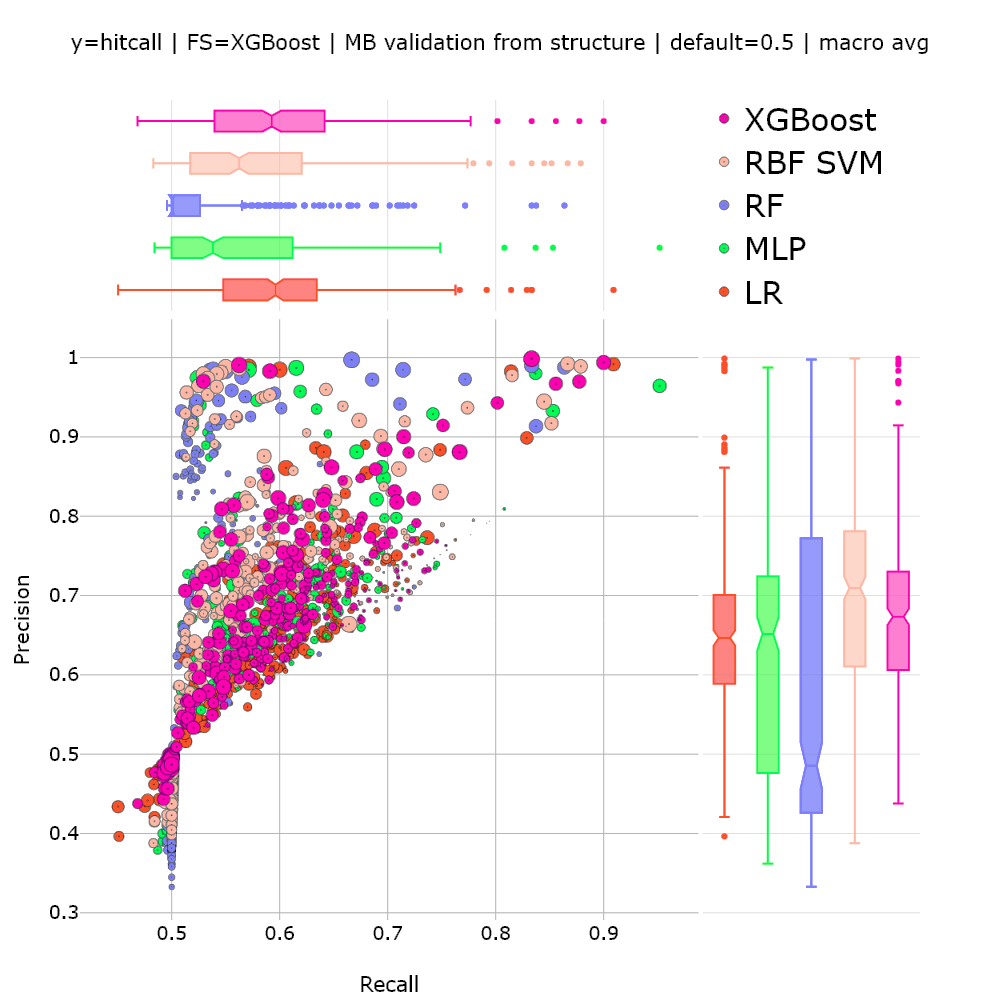
\includegraphics[width=\textwidth]{generated_results/hitcall_classification_Feature_Selection_XGBClassifier_mb_val_structure_default_macro_avg.png}
      \caption{}
  \label{fig:hitcall_classification_Feature_Selection_XGBClassifier_mb_val_structure_default_macro_avg}
  \end{subfigure}
  \hfill
  \begin{subfigure}[b]{0.495\textwidth}
      \centering
      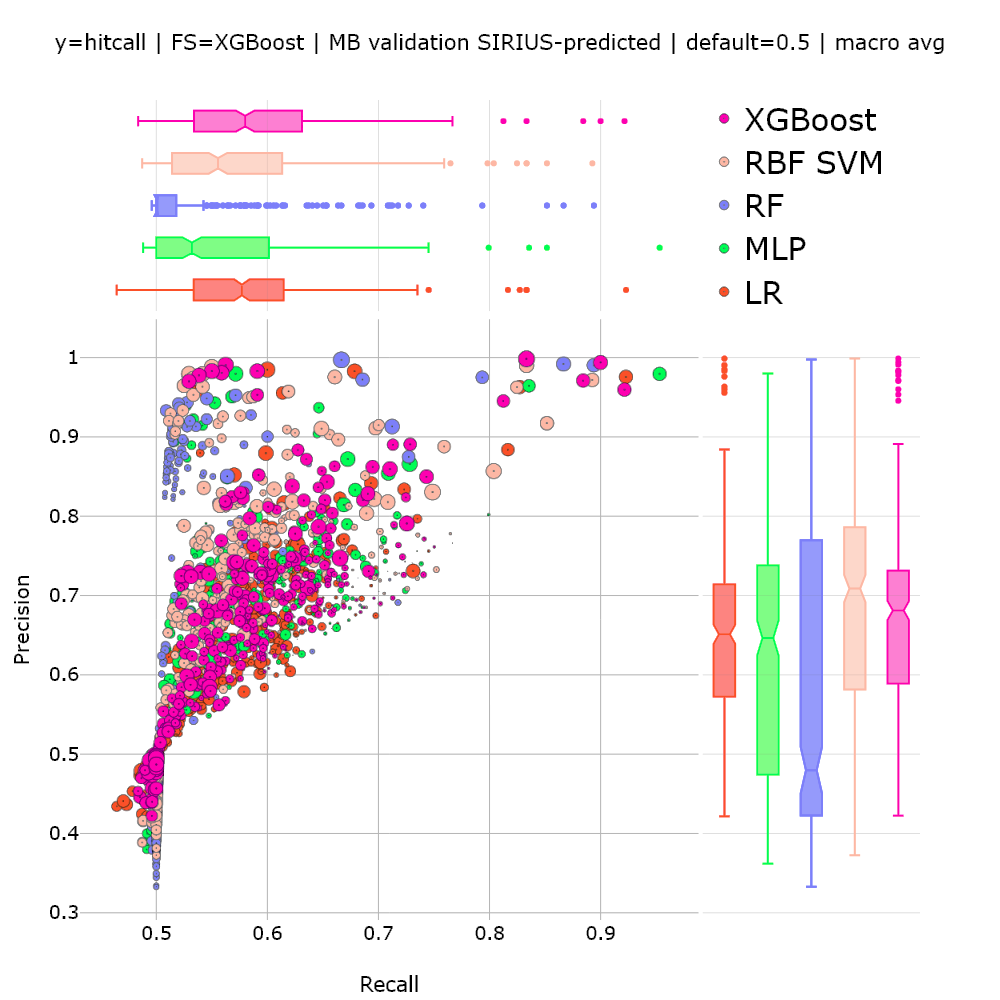
\includegraphics[width=\textwidth]{generated_results/hitcall_classification_Feature_Selection_XGBClassifier_mb_val_sirius_default_macro_avg.png}
      \caption{}
      \label{fig:hitcall_classification_Feature_Selection_XGBClassifier_mb_val_sirius_default_macro_avg}
  \end{subfigure}
  \caption{Comparison of Precision and Recall for five different estimators across all evaluated assay endpoints. MassBank Validation Set with fingerprints from chemical structure (a) and SIRIUS-predicted fingerprints (b), $default$ threshold, macro averaged metrics. Larger marker size indicate the larger relative imbalance between the support for negative and positive compounds, normalized across all assay endpoints. The marginal boxplots illustrate the distribution of the performance metrics across the target assay endpoint models (median, first quartile (Q1), third quartile (Q3), whiskers (range) and outlieres). The tables below provide the average metrics for the estimators across all target assay endpoint models.}
  \label{fig:hitcall_classification_Feature_Selection_XGBClassifier_mb_val_default_macro_avg}
\end{figure}

\begin{longtable}{llllllll}
\caption{Median Performance Metrics belonging to Figure~\ref{fig:hitcall_classification_Feature_Selection_XGBClassifier_mb_val_structure_default_macro_avg}.}\label{tab:table:hitcall_classification_feature_selection_xgbclassifier_mb_val_structure_default_macro_avg}\\
\toprule
\midrule
\small Estimator & \small Precision & \small Recall & \small F1 & \small Acc. & \small Bal. Acc. & \small ROC-AUC & \small PR-AUC\\
\hline
LR & 0.647 & 0.596 & 0.605 & 0.816 & 0.596 & 0.707 & 0.411\\
MLP & 0.651 & 0.538 & 0.530 & 0.829 & 0.538 & 0.671 & 0.363\\
RBF SVM & 0.709 & 0.562 & 0.570 & 0.835 & 0.562 & 0.738 & 0.455\\
RF & 0.486 & 0.500 & 0.474 & 0.829 & 0.500 & 0.731 & 0.436\\
XGBoost & 0.673 & 0.593 & 0.607 & 0.823 & 0.593 & 0.736 & 0.451\\
\bottomrule
\end{longtable}

\begin{longtable}{llllllll}
\caption{Median Performance Metrics belonging to~\ref{fig:hitcall_classification_Feature_Selection_XGBClassifier_mb_val_sirius_default_macro_avg}.}\label{tab:table:hitcall_classification_feature_selection_xgbclassifier_mb_val_sirius_default_macro_avg}\\
\toprule
\midrule
\small Estimator & \small Precision & \small Recall & \small F1 & \small Acc. & \small Bal. Acc. & \small ROC-AUC & \small PR-AUC\\
\hline
LR & 0.651 & 0.577 & 0.587 & 0.820 & 0.577 & 0.693 & 0.385\\
MLP & 0.646 & 0.532 & 0.519 & 0.829 & 0.532 & 0.668 & 0.355\\
RBF SVM & 0.709 & 0.556 & 0.559 & 0.834 & 0.556 & 0.726 & 0.448\\
RF & 0.480 & 0.500 & 0.471 & 0.829 & 0.500 & 0.727 & 0.433\\
XGBoost & 0.681 & 0.580 & 0.594 & 0.829 & 0.580 & 0.721 & 0.441\\
\bottomrule
\end{longtable}

\newpage

\begin{figure}
  \centering
  \begin{subfigure}[b]{0.495\textwidth}
      \centering
      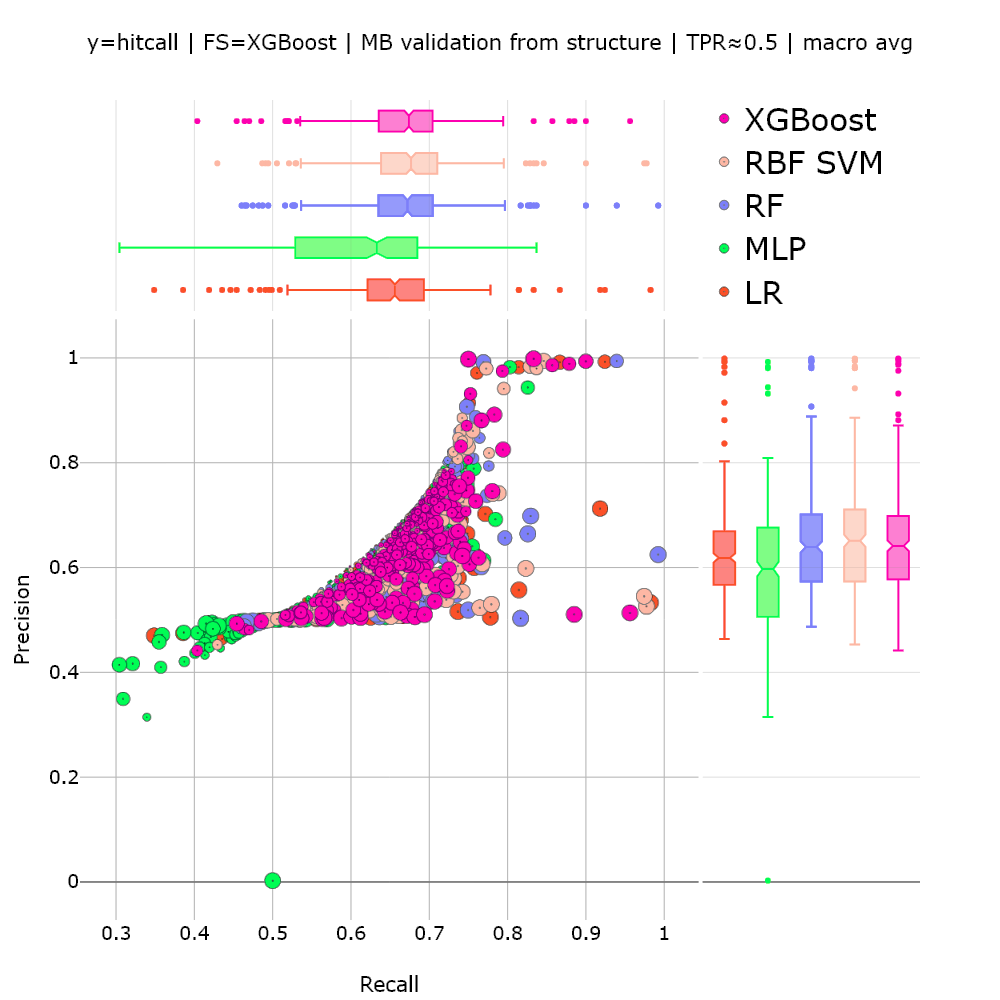
\includegraphics[width=\textwidth]{generated_results/hitcall_classification_Feature_Selection_XGBClassifier_mb_val_structure_tpr_macro_avg.png}
      \caption{}
  \label{fig:hitcall_classification_Feature_Selection_XGBClassifier_mb_val_structure_tpr_macro_avg}
  \end{subfigure}
  \hfill
  \begin{subfigure}[b]{0.495\textwidth}
      \centering
      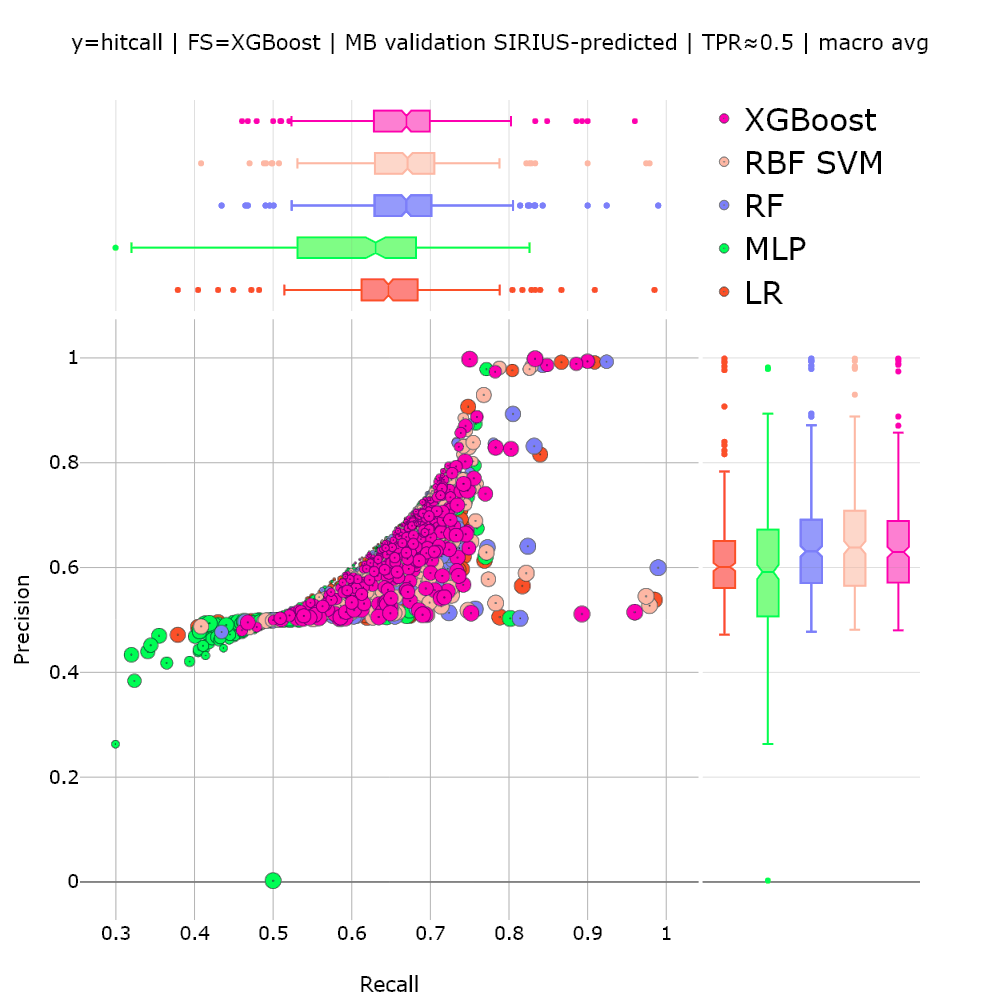
\includegraphics[width=\textwidth]{generated_results/hitcall_classification_Feature_Selection_XGBClassifier_mb_val_sirius_tpr_macro_avg.png}
      \caption{}
      \label{fig:hitcall_classification_Feature_Selection_XGBClassifier_mb_val_sirius_tpr_macro_avg}
  \end{subfigure}
  \caption{Comparison of Precision and Recall for five different estimators across all evaluated assay endpoints. MassBank Validation Set with fingerprints from chemical structure (a) and SIRIUS-predicted fingerprints (b), $TPR \simeq 0.5$ threshold, macro averaged metrics.}
  \label{fig:hitcall_classification_Feature_Selection_XGBClassifier_mb_val_tpr_macro_avg}
\end{figure}

\begin{longtable}{llllllll}
\caption{Median Performance Metrics belonging to Figure~\ref{fig:hitcall_classification_Feature_Selection_XGBClassifier_mb_val_structure_tpr_macro_avg}.}\label{tab:table:hitcall_classification_feature_selection_xgbclassifier_mb_val_structure_tpr_macro_avg}\\
\toprule
\midrule
\small Estimator & \small Precision & \small Recall & \small F1 & \small Acc. & \small Bal. Acc. & \small ROC-AUC & \small PR-AUC\\
\hline
LR & 0.618 & 0.656 & 0.626 & 0.727 & 0.596 & 0.707 & 0.411\\
MLP & 0.597 & 0.633 & 0.605 & 0.683 & 0.538 & 0.671 & 0.363\\
RBF SVM & 0.651 & 0.677 & 0.656 & 0.754 & 0.562 & 0.738 & 0.455\\
RF & 0.639 & 0.672 & 0.647 & 0.750 & 0.500 & 0.731 & 0.436\\
XGBoost & 0.641 & 0.674 & 0.649 & 0.754 & 0.593 & 0.736 & 0.451\\
\bottomrule
\end{longtable}

\begin{longtable}{llllllll}
\caption{Median Performance Metrics belonging to Figure~\ref{fig:hitcall_classification_Feature_Selection_XGBClassifier_mb_val_sirius_tpr_macro_avg}.}\label{tab:table:hitcall_classification_feature_selection_xgbclassifier_mb_val_sirius_tpr_macro_avg}\\
\toprule
\midrule
\small Estimator & \small Precision & \small Recall & \small F1 & \small Acc. & \small Bal. Acc. & \small ROC-AUC & \small PR-AUC\\
\hline
LR & 0.601 & 0.647 & 0.608 & 0.711 & 0.577 & 0.693 & 0.385\\
MLP & 0.592 & 0.630 & 0.596 & 0.676 & 0.532 & 0.668 & 0.355\\
RBF SVM & 0.638 & 0.671 & 0.644 & 0.749 & 0.556 & 0.726 & 0.448\\
RF & 0.631 & 0.669 & 0.638 & 0.743 & 0.500 & 0.727 & 0.433\\
XGBoost & 0.629 & 0.670 & 0.638 & 0.743 & 0.580 & 0.721 & 0.441\\
\bottomrule
\end{longtable}

\newpage

\begin{figure}[htbp]
  \centering
  \begin{subfigure}[b]{0.495\textwidth}
      \centering
      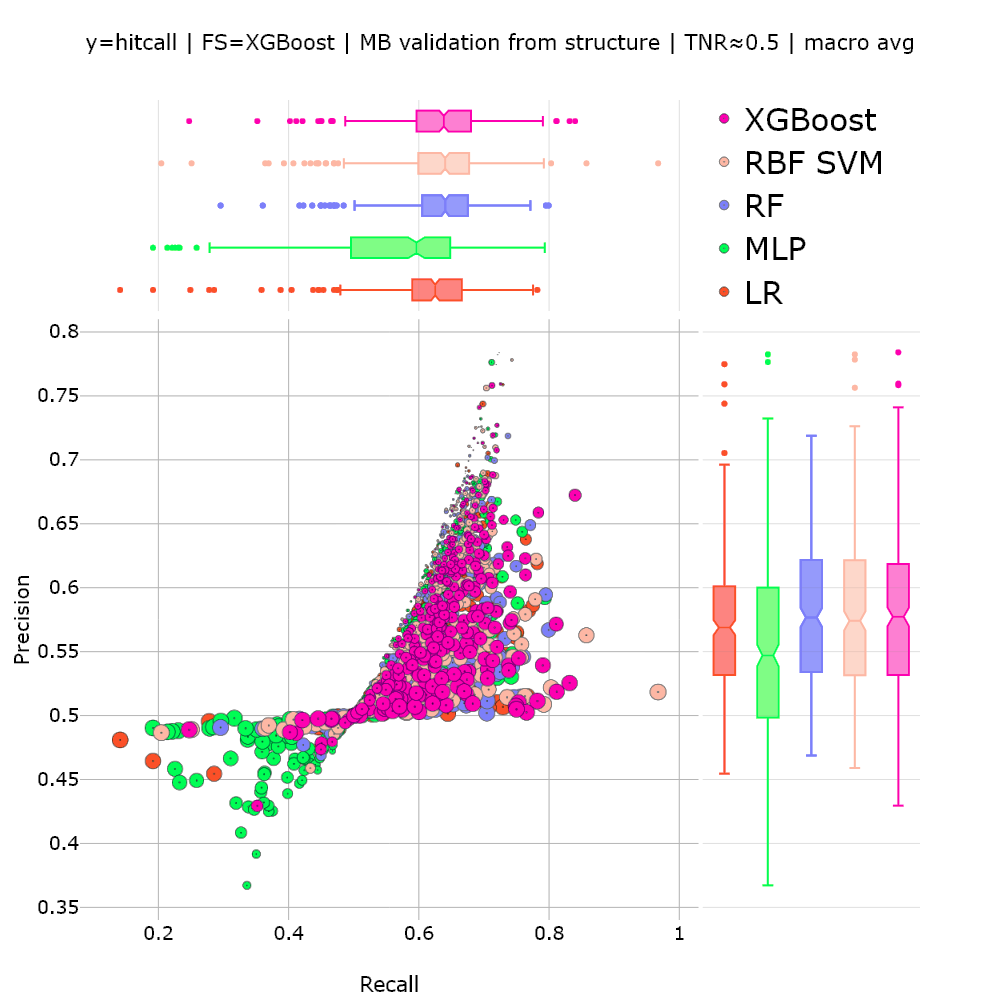
\includegraphics[width=\textwidth]{generated_results/hitcall_classification_Feature_Selection_XGBClassifier_mb_val_structure_tnr_macro_avg.png}
      \caption{}
  \label{fig:hitcall_classification_Feature_Selection_XGBClassifier_mb_val_structure_tnr_macro_avg}
  \end{subfigure}
  \hfill
  \begin{subfigure}[b]{0.495\textwidth}
      \centering
      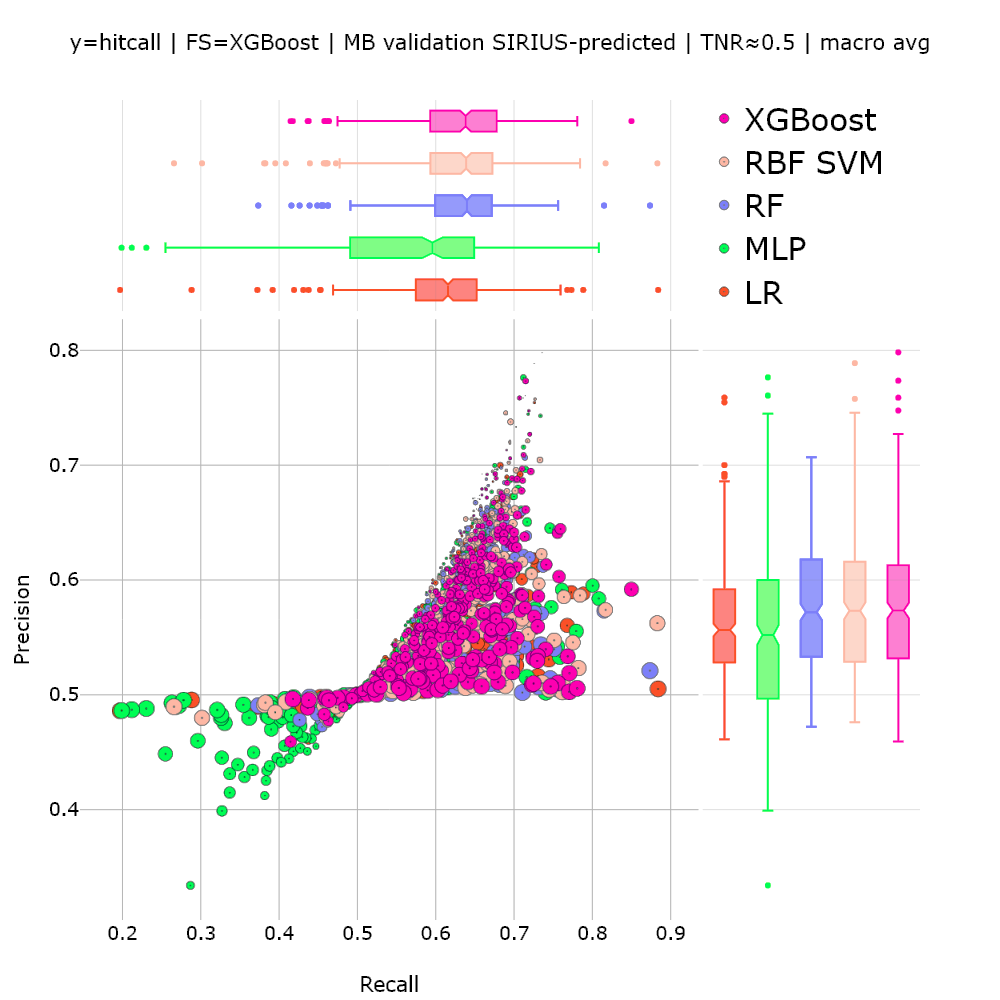
\includegraphics[width=\textwidth]{generated_results/hitcall_classification_Feature_Selection_XGBClassifier_mb_val_sirius_tnr_macro_avg.png}
      \caption{}
      \label{fig:hitcall_classification_Feature_Selection_XGBClassifier_mb_val_sirius_tnr_macro_avg}
  \end{subfigure}
  \caption{Comparison of Precision and Recall for five different estimators across all evaluated assay endpoints. MassBank Validation Set with fingerprints from chemical structure (a) and SIRIUS-predicted fingerprints (b), $TNR \simeq 0.5$ threshold, macro averaged metrics.}
  \label{fig:hitcall_classification_Feature_Selection_XGBClassifier_mb_val_tnr_macro_avg}
\end{figure}

\begin{longtable}{llllllll}
\caption{Median Performance Metrics belonging to Figure~\ref{fig:hitcall_classification_Feature_Selection_XGBClassifier_mb_val_structure_tnr_macro_avg}.}\label{tab:table:hitcall_classification_feature_selection_xgbclassifier_mb_val_structure_tnr_macro_avg}\\
\toprule
\midrule
\small Estimator & \small Precision & \small Recall & \small F1 & \small Acc. & \small Bal. Acc. & \small ROC-AUC & \small PR-AUC\\
\hline
LR & 0.569 & 0.625 & 0.509 & 0.552 & 0.596 & 0.707 & 0.411\\
MLP & 0.547 & 0.596 & 0.478 & 0.537 & 0.538 & 0.671 & 0.363\\
RBF SVM & 0.574 & 0.640 & 0.509 & 0.556 & 0.562 & 0.738 & 0.455\\
RF & 0.577 & 0.641 & 0.514 & 0.555 & 0.500 & 0.731 & 0.436\\
XGBoost & 0.577 & 0.638 & 0.509 & 0.553 & 0.593 & 0.736 & 0.451\\
\bottomrule
\end{longtable}

\begin{longtable}{llllllll}
\caption{Median Performance Metrics belonging to~\ref{fig:hitcall_classification_Feature_Selection_XGBClassifier_mb_val_sirius_tnr_macro_avg}.}\label{tab:table:hitcall_classification_feature_selection_xgbclassifier_mb_val_sirius_tnr_macro_avg}\\
\toprule
\midrule
\small Estimator & \small Precision & \small Recall & \small F1 & \small Acc. & \small Bal. Acc. & \small ROC-AUC & \small PR-AUC\\
\hline
LR & 0.557 & 0.616 & 0.497 & 0.543 & 0.577 & 0.693 & 0.385\\
MLP & 0.552 & 0.596 & 0.481 & 0.541 & 0.532 & 0.668 & 0.355\\
RBF SVM & 0.573 & 0.639 & 0.506 & 0.555 & 0.556 & 0.726 & 0.448\\
RF & 0.572 & 0.640 & 0.507 & 0.553 & 0.500 & 0.727 & 0.433\\
XGBoost & 0.573 & 0.638 & 0.507 & 0.553 & 0.580 & 0.721 & 0.441\\
\bottomrule
\end{longtable}
\newpage


\begin{figure}[htbp]
  \centering
  \begin{subfigure}[b]{0.495\textwidth}
      \centering
      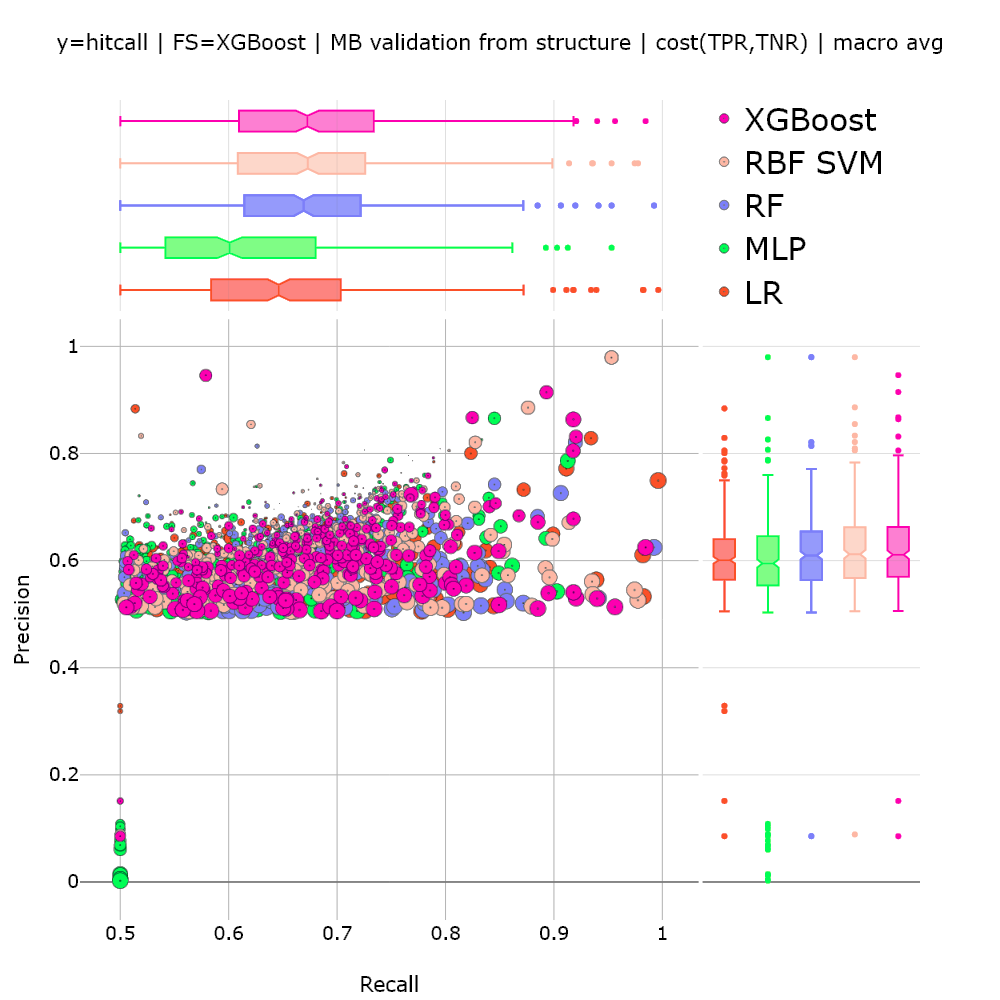
\includegraphics[width=\textwidth]{generated_results/hitcall_classification_Feature_Selection_XGBClassifier_mb_val_structure_optimal_macro_avg.png}
      \caption{}
  \label{fig:hitcall_classification_Feature_Selection_XGBClassifier_mb_val_structure_optimal_macro_avg}
  \end{subfigure}
  \hfill
  \begin{subfigure}[b]{0.495\textwidth}
      \centering
      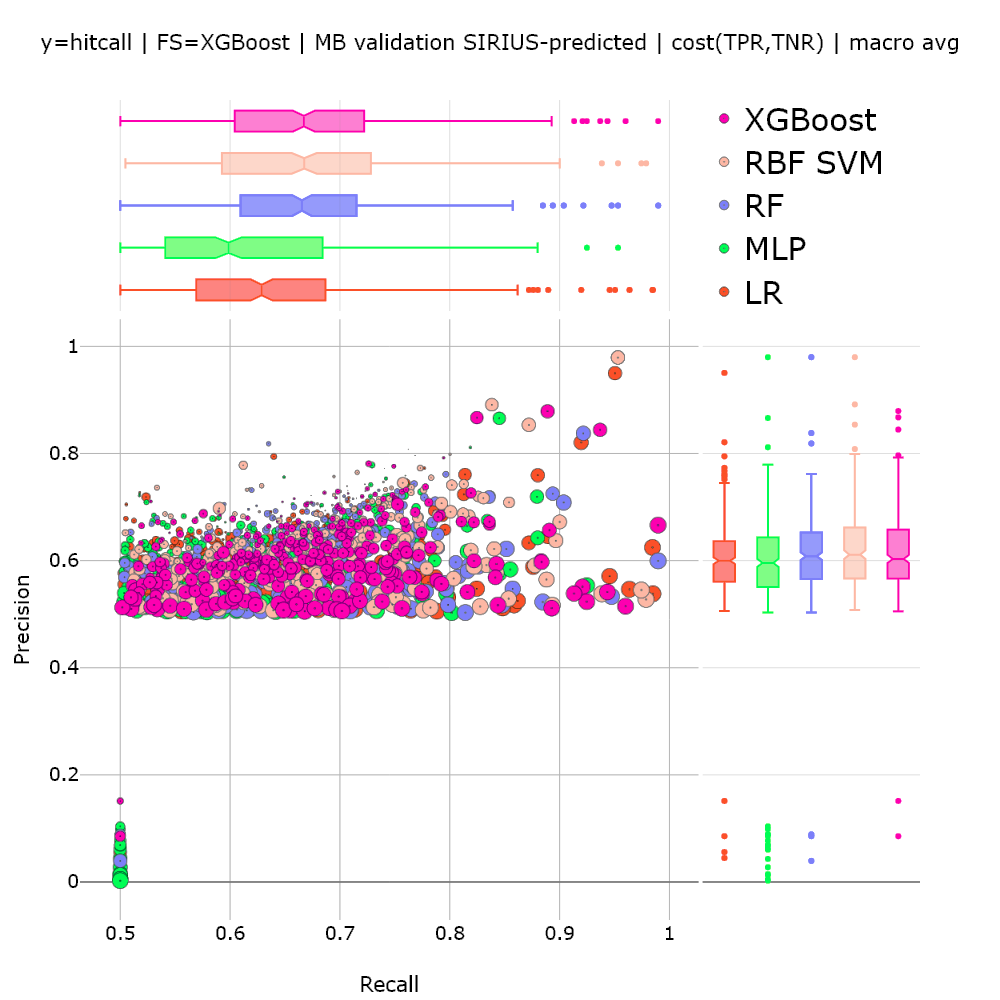
\includegraphics[width=\textwidth]{generated_results/hitcall_classification_Feature_Selection_XGBClassifier_mb_val_sirius_optimal_macro_avg.png}
      \caption{}
      \label{fig:hitcall_classification_Feature_Selection_XGBClassifier_mb_val_sirius_optimal_macro_avg}
  \end{subfigure}
  \caption{Comparison of Precision and Recall for five different estimators across all evaluated assay endpoints. MassBank Validation Set with fingerprints from chemical structure (a) and SIRIUS-predicted fingerprints (b), $\text{cost}(TPR, TNR) = 2 * (1 - TPR) + FPR$ threshold, macro averaged metrics.}
  \label{fig:hitcall_classification_Feature_Selection_XGBClassifier_mb_val_optimal_macro_avg}
\end{figure}

\begin{longtable}{llllllll}
\caption{Median Performance Metrics belonging to Figure~\ref{fig:hitcall_classification_Feature_Selection_XGBClassifier_mb_val_structure_optimal_macro_avg}.}\label{tab:table:hitcall_classification_feature_selection_xgbclassifier_mb_val_structure_optimal_macro_avg}\\
\toprule
\midrule
\small Estimator & \small Precision & \small Recall & \small F1 & \small Acc. & \small Bal. Acc. & \small ROC-AUC & \small PR-AUC\\
\hline
LR & 0.601 & 0.646 & 0.470 & 0.503 & 0.596 & 0.707 & 0.411\\
MLP & 0.595 & 0.601 & 0.386 & 0.407 & 0.538 & 0.671 & 0.363\\
RBF SVM & 0.612 & 0.673 & 0.516 & 0.559 & 0.562 & 0.738 & 0.455\\
RF & 0.610 & 0.669 & 0.507 & 0.548 & 0.500 & 0.731 & 0.436\\
XGBoost & 0.611 & 0.673 & 0.511 & 0.563 & 0.593 & 0.736 & 0.451\\
\bottomrule
\end{longtable}

\begin{longtable}{llllllll}
\caption{Median Performance Metrics belonging to~\ref{fig:hitcall_classification_Feature_Selection_XGBClassifier_mb_val_sirius_optimal_macro_avg}.}\label{tab:table:hitcall_classification_feature_selection_xgbclassifier_mb_val_sirius_optimal_macro_avg}\\
\toprule
\midrule
\small Estimator & \small Precision & \small Recall & \small F1 & \small Acc. & \small Bal. Acc. & \small ROC-AUC & \small PR-AUC\\
\hline
LR & 0.600 & 0.629 & 0.432 & 0.458 & 0.577 & 0.693 & 0.385\\
MLP & 0.596 & 0.599 & 0.373 & 0.415 & 0.532 & 0.668 & 0.355\\
RBF SVM & 0.611 & 0.668 & 0.493 & 0.559 & 0.556 & 0.726 & 0.448\\
RF & 0.608 & 0.665 & 0.499 & 0.534 & 0.500 & 0.727 & 0.433\\
XGBoost & 0.603 & 0.667 & 0.502 & 0.539 & 0.580 & 0.721 & 0.441\\
\bottomrule
\end{longtable}
% \subsection{Feature Importance}

\section{Discussion}









